\section{Summary of Stein variational gradient descent} \label{sec:summary}
\emph{Stein variational gradient descent} (SVGD) \citep{liu2016stein} is a particle-based variational inference method, which iteratively transforms a set of samples from a reference distribution to the target distribution. In general, SVGD only requires the gradient of the log density function of the target distribution. This fits well into the framework of Bayesian inference, which usually has intractable normalizing constant in target distribution.   Comparing to traditional sampling methods such as Markov Chain Monte Carlo (MCMC), SVGD uses deterministic updates and does not experience slow convergence due to autocorrelation between samples. A big advantage is that it leverage the gradient information of the target distribution, However, it also has many shortcomings. In this section, we briefly summarize the development of SVGD  and its underlying theory, and discuss its limitations at the end of this section.



\subsection{KL minimization and Stein's operator}

Similar to normalizing flow \citep{kobyzev2020normalizing}, SVGD aims to learn an invertible transformation from a reference distribution to the target distribution $p$.
Instead of composing a series of parametric functions and optimizing over all the parameters, SVGD iteratively performs a non-parametric transformation to the current distribution and decreases the KL divergence to the target.

Let $X $ be a random variable follows a distribution with density function $q(x)$, which dominates $p$.  Let $T: \reals^d \to \reals^d$ be an invertible and continuously differentiable map.  In particular, we focus on the perturbed identity map:
\[
    T(x) \defined x + \eps \phi(x) , \quad \phi \in \mcH_k^d \text{ and } \phi \text{ is smooth}.
\] 
Here $\mcH_k^d$ is a \emph{Reproducing kernel Hilbert space}(RKHS), a Hilbert space induced by a positive definite kernel $\kappa(x, x'): \reals^d\times \reals^d \to \reals$.  We denote $q_T$ as the push forward measure of $Y \defined T(X)$, of which the density function can be written as 
\[
q_T(y) = q\left(T^{-1}(y)\right)\cdot \left| \det \nabla T^{-1}(y) \right|.
\]
The development of SVGD arise from a critical connection between the KL divergence and the \emph{Stein's operator}. 

Considering the directional derivative of $\kl{q_T}{p}$ along $\phi \in \mcH_k^d$,
\[
\left. \der{}{\eps} \kl{q_T}{p} \right|_{\eps = 0} &= -\int q(x) \left( \nabla \log p(x)^T \phi(x)  - \tr \nabla\phi(x) \right)\\
& = -\EE_{q}\left[ \nabla \log p(X)^T \phi(X)  + \tr \nabla\phi(X) \right].
\]
A key observation here is that $\nabla \log p(X)^T \phi(X)  + \tr \nabla\phi(X)$ is the \emph{Stein operator} applied to $\phi(x)$.
Then since $\phi \in \mcH_k^d$, the reproducing property of the kernel $\kappa(\cdot, \cdot)$ yields that  
\[
    \left. \der{}{\eps} \kl{q}{p} \right|_{\eps = 0}  = - \left\langle \phi, \EE_{q}\left[ \kappa(x, \cdot) \nabla \log p(X)^T \phi(X)  + \nabla_x \kappa(x,\cdot ) \right] \right\rangle_{\mcH_k^d}.
\] 
Note that the gradient is the directional derivative along the steepest descent direction.   By maximizing the right hand side over $\phi  \in \mcH_k^d$, we obtain that
\[
    & \phi^\star(\cdot) = \EE_{q}\left[ \kappa(x, \cdot) \nabla \log p(X)^T \phi(X)  + \nabla \kappa(x,\cdot ) \right], \quad \text{and} \label{eq:optimaldirection}\\
    & \left. \nabla_\eps \kl{q}{p} \right|_{\eps = 0}  = \|\phi^\star\|_{\mcH_k^d}^2 = \dee_{\kappa}(q, p). \label{eq:KLgrad}
\]
Here $\dee_{\kappa}(q, p)$ is the \emph{kernelized Stein discrepancy} between $q$ and $p$. Thus, by iteratively applying the following transformation to $X_0$,
\[\label{eq:normflow}
X_0\sim q_0, \quad X_{k+1} &\gets T(X_k),\quad  T(X_k) \defined X_k + \eps \phi^\star(X_k), \quad k=0, 1 ,\dots.
\] 
We are able to construct a non-parametric normalizing flow that decreases the KL-divergence sequentially. As revealed in \cref{eq:KLgrad}, the fixed point of this transformation is achieved if and only if $ \dee_{\kappa}(q, p) = 0$. It is worth pointing out that in general $ \dee_{\kappa}(q, p) = 0$ does not imply that $q = p$. In fact, this requires a proper choice of the kernel function $\kappa(\cdot, \cdot)$, which will be discussed in detail in \cref{sec:kernelchoice}.

To implement this non-parametric normalizing flow \cref{eq:normflow}, \citet{liu2016stein} approximate the optimal direction \cref{eq:optimaldirection} using Monte Carlo samples.
Specifically, one may draw $n$ samples $\{x_i^{(0)}  \}_{i = 1}^n$  from the reference distribution $p_0$ and apply the empirical version of \cref{eq:normflow} to the set of particles, i.e., for $i = 0, 1,\dots, n$ and learning rate $\gamma_k >0$,  the numerical iteration at $k$-th iteration is as follows,
\[
   \begin{aligned}
    x_{i}^{(k+1)} & \leftarrow x_{i}^{(k)}+ \gamma_k \hat{\phi}_k^{\star}\left(x_{i}^{(k)}\right),\quad \text {where } \\
    \hat{\phi}_k^{\star}(x) & \defined \frac{1}{n} \sum_{j=1}^{n}\left[\kappa\left(x_{j}^{(k)}, x\right) \nabla \log p\left(x_{j}^{(k)}\right)+\nabla_{x_{j}^{(k)}} \kappa\left(x_{j}^{(k)}, x\right)\right].
   \end{aligned}
   \label{eq:svgd}
\]
Ideally, this iterative procedure will move the set of particle to the target distribution, which will eventually produce samples from $p$.  The detailed description of the standard SVGD is presented in \cref{alg:SVGD}.
In practice, to achieve a faster numerical convergence, \citet{liu2016stein} suggest using the AdaGrad updates with momentum---also known as RMSprop--- instead of vanilla gradient descent update described in \cref{eq:svgd}.  
Specifically, RMSprop performs the update at $k$-th iteration as follows: for $i = 1, 2, \dots, n$,
\[\label{eq:rms}
    \begin{aligned}
        g_{k+1} &\gets \eta g_k + (1 - \eta) \left(\hat{\phi}_k^{\star}\left(x_{i}^{(k)}\right)\right)^2,\\
        x_{i}^{(k+1)} &\gets x_i^{(k)} + \frac{\gamma_k}{\sqrt{g_{k+1}+\eps} } \hat{\phi}_k^{\star}\left(x_{i}^{(k)}\right),  
    \end{aligned}  
\]
where $g_0 = 0\cdot\ind$ and all operations on vectors are elementwise. By default, the momentum factor $\eta$ is set to $0.9$ and the smoothing factor $\eps$ is set to $10^{-8}$. Empirically, we do observe significantly faster convergence of the above update rule than the naive gradient descent update \cref{eq:svgd}. 







\subsection{Choice of the kernel} \label{sec:kernelchoice}

Although we have formulated the construction of SVGD algorithm using some nice properties of RKHS, we have not provided any guideline of the selection of $\kappa(\cdot, \cdot)$. Note that the behaviour of SVGD is strongly dependent on the choice of the kernel.  Therefore, it is helpful to understand the fundamental requirements of the kernel function.

Recall the transformation $T$ described in \cref{eq:normflow}, which is considered to be invertible and differentiable. By the Hadmard's global inverse function theorem, a sufficient condition for the invertibility of $T$ is to have a bounded kernel function. 
Another concern on the kernel is related to the converging point of \cref{eq:normflow} as $k \to \infty$. As we mentioned above, the process of \cref{eq:normflow} will converge to a fixed point of the transformation $T$, where kernelized Stein discrepancy between the current distribution $q$ and the target distribution $p$ arrives at 0. Ideally, we want to have $d_\kappa(q ,p) = 0$ if and only if $q = p$. A sufficient condition for this is that $\kappa(\cdot, \cdot)$ is \emph{integrally strictly positive definition} \citep{liu2016kernelized}, i.e., 
\[
\forall  0<\|g\|_{2}^{2}<\infty, \quad    \int_{\mathcal{X}} g(x) k\left(x, x^{\prime}\right) g\left(x^{\prime}\right) \dee x \dee x^{\prime}>0.    
\]

Examples of kernels satisfying these two properties are given by  
\[
\forall (x, x')\in \reals\times \reals,\quad  \kappa(x, x'; h) = \exp\left( -\frac{1}{h} |x - x'|^p \right),  \quad p \in(0, 2].
\]
When $p = 2$, this yields the RBFkernel. Here $h> 0$ denotes the bandwidth of the kernel, which is a critical hyperparameter. 

Different values of the kernel bandwidth can significantly influence the quality of SVGD; users need to hand tune the bandwidth to optimize the performance of SVGD. When using RBF  kernel, \citet{liu2016stein} suggests picking the bandwidth based on the median of the pairwise Euclidean distances between the current particles, i.e., $h=\operatorname{med}^{2} / \log n$, where $\operatorname{med}$ is the median of the Euclidean distances. This procedure will update the bandwidth automatically at each iteration and works generally well. However, we will show in \cref{sec:asvgd} when the median trick can be problematic.




\captionsetup[subfigure]{labelformat=empty}
\begin{figure}[t!]
    \centering 
\begin{subfigure}[b]{.48\textwidth} 
    \scalebox{1}{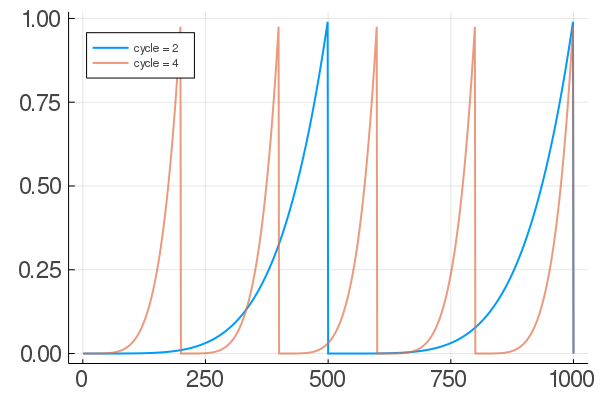
\includegraphics[width=\textwidth]{figures/Asched_c.png}}
    \caption{(a)\label{fig:aschedc}}
\end{subfigure}
\hfill
\centering
\begin{subfigure}[b]{0.48\textwidth}
    \scalebox{1}{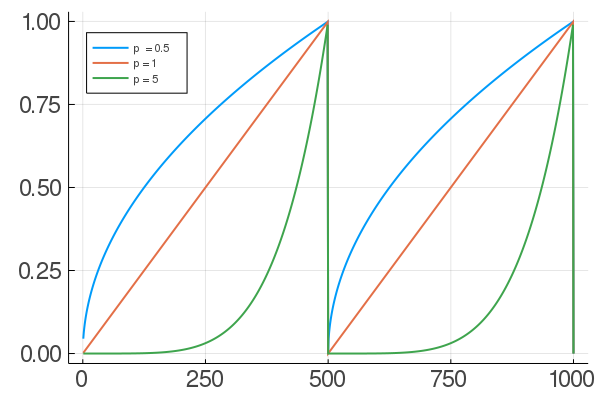
\includegraphics[width=\textwidth]{figures/Asched_p.png}}
    \caption{(b)\label{fig:aschedp}}
\end{subfigure}

\caption{Annealing schedules. \cref{fig:aschedc} shows two annealing schedules with $2$ cycles and $4$ cycles respectively. \cref{fig:aschedp} shows annealing schedules across $p  = 0.5, 1, 5$.}
\label{fig:acsched}
\end{figure}




\captionsetup[subfigure]{labelformat=empty}
\begin{figure}[t!]
    \centering 
\begin{subfigure}[b]{.48\textwidth} 
    \scalebox{1}{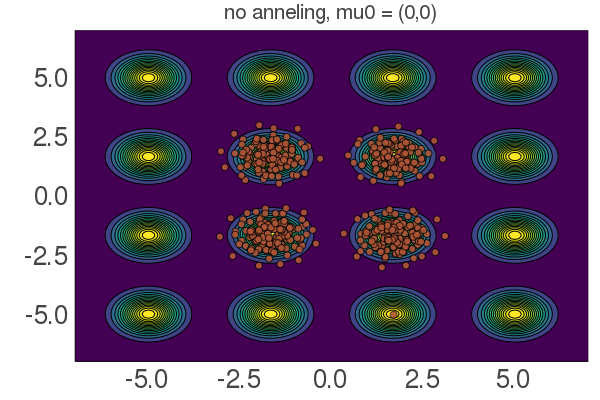
\includegraphics[width=\textwidth]{figures/T0_rms.png}}
    \caption{(a)\label{fig:T0_rms}}
\end{subfigure}
\hfill
\centering
\begin{subfigure}[b]{0.48\textwidth}
    \scalebox{1}{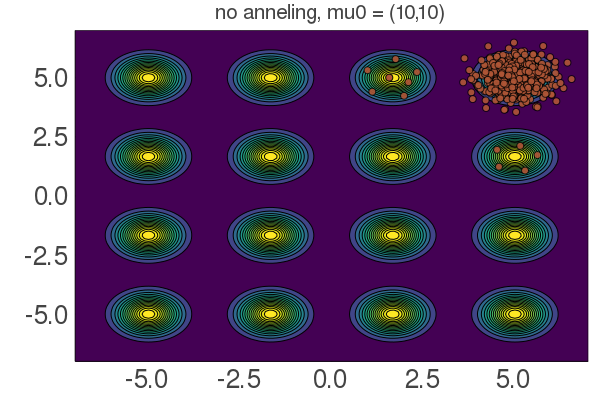
\includegraphics[width=\textwidth]{figures/T10_rms.png}}
    \caption{(b)\label{fig:T10_rms}}
\end{subfigure}
\hfill
\centering
\begin{subfigure}[b]{.48\textwidth} 
    \scalebox{1}{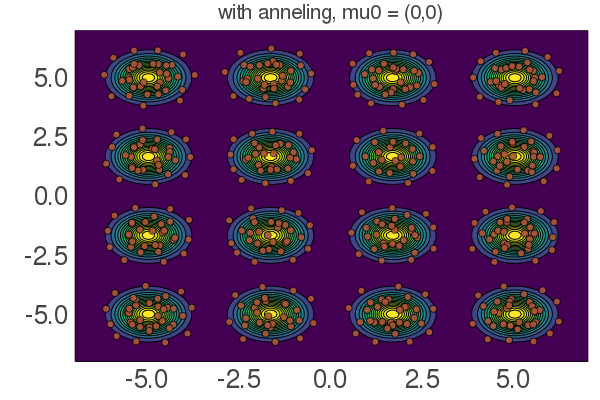
\includegraphics[width=\textwidth]{figures/T0_rms_anneal.png}}
    \caption{(c)\label{fig:T0_rms_anneal}}
\end{subfigure}
\hfill
\centering
\begin{subfigure}[b]{0.48\textwidth}
    \scalebox{1}{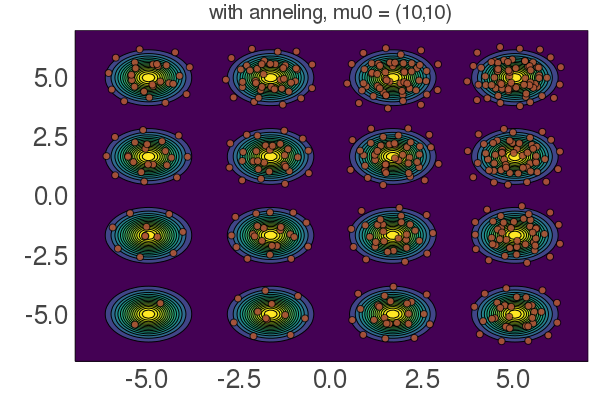
\includegraphics[width=\textwidth]{figures/T10_rms_anneal.png}}
    \caption{(d)\label{fig:T10_rms_anneal}}
\end{subfigure}
\caption{Comparison of SVGD (\cref{fig:T0_rms,fig:T10_rms}) and A-SVGD (\cref{fig:T0_rms_anneal,fig:T10_rms_anneal}) on the synthetic Gaussian mixture with 16 components with $\sigma = 0.5$ across two set of initial particles. }
\label{fig:SVGD_ASVGD}
\end{figure}









\subsection{Limitations of SVGD} 

A key limitation of SVGD is its
computational burden. Note that the deterministic updates described in \cref{eq:svgd} require the
evaluation of the kernel matrix and its gradient, which costs $\mcO(n^2)$.
This makes SVGD less practical compared to other particle sampling methods
such as sequential Monte Carlo sampler---which costs $\mcO(n)$---if we aim to
obtain a large number of samples from the target distribution.

The computation problem also occurs when calculating the gradient $\nabla log
p(x)$ for all particles; this is particularly expensive in a large dataset
setting. Considering the target distribution as the posterior distribution
of a Bayesian model, i.e., $p(\theta) \propto \pi_0(\theta)\prod_{i = 1}^{m}
p(x_i \mid \theta)$ where $\pi_0$ denotes the prior distribution of $\theta$,
computing $\nabla \log p(\theta)$ exactly is not practical as $m$ is large.
Stochastic gradient estimates using subsampled data points can be applied in this case to make SVGD scalable.


In the following sections, we focus on another common issue of SVGD when the target
distribution $p(x)$ has multiple modes: the mixing problem, where the
particles collapse at a particular mode of the target distribution and fail
to distribute the particles to other high density regions. This is also known
as the \emph{mode collapse} phenomenon \citep{zhuo2018message,d2021annealed}
and appears often when the modes are distant from each other. The problem of
mode collapsing tends to be more severe in high-dimensional settings, but can
also be observed on a simple 2D Gaussian mixture target. Variants of SVGD are developed to resolve this issue (or at least alleviate the problem). 
For example, \citet{d2021annealed} adopts the tempering method from the MCMC literature \citep{zhang2019cyclical} that includes an annealing schedule in the SVGD updates; 
\citet{zhuo2018message} leverages the latent structure of the statistical model and converts the inference problem into a lower-dimensional space. 

In the next section,
we provide a clear illustration of the mixing issue on two synthetic examples
and introduce the annealed Stein variational gradient descent (A-SVGD), which tends to reduce the mixing issue. 
Further, we identify a central problem regarding the kernel bandwidth, which inspires our idea in \cref{sec:bw}.




